\subsection{Informative delays and partial outcomes}
\label{sec:async_exp}
A separate frozen simulation isolates an asymmetric measurement pipeline.
Both systems succeed with probability 0.90; their lognormal cost scales
are equal under the null and have ratio 0.55 under the alternative.
Failures and expensive traces from $A$ are reported late, even when the
systems have identical outcome distributions. We enroll 100 pairs per
tick, up to 6,000, and reveal all outcomes within 20 ticks of enrollment.
This directly simulates the balanced oriented score law, without running
agents or assigning production users. Each of 1,000 repetitions per
scenario is shared by three methods: completed-only selection, completed
prefixes, and partial-score prefix inference. The two valid methods use
the same candidate prefixes, positive bets, and same-prefix conjunction
of preference superiority and success noninferiority at margin 0.03.
Missing bits admit both outcomes; unrevealed cost signs admit all signs.
The bounds do not infer hidden values from the informative reveal clock.

Under identical outcomes, completed-only selection falsely deployed in
1000 of 1,000 repetitions, whereas each valid method
deployed in 6 (0.6\%; Wilson 95\% interval,
0.275--1.303\%).
Under the cheaper alternative, both valid methods deployed in
997 of 1,000 repetitions.
Partial evidence reduced mean capped decision time from
41.285 to 22.363 ticks;
the paired gain was 18.922
(Monte Carlo standard error 0.033).
Mean initiated executions fell from
8130.8 to 4459.6.
No partial decision occurred later than its comparator, and all
997 deployment paths were strictly earlier.
Identical final decisions after complete revelation are guaranteed by
the matched prefix construction, not evidence of universally high power.
The magnitude of the gain depends on this particular reveal mechanism.

\begin{figure}[t]
\centering
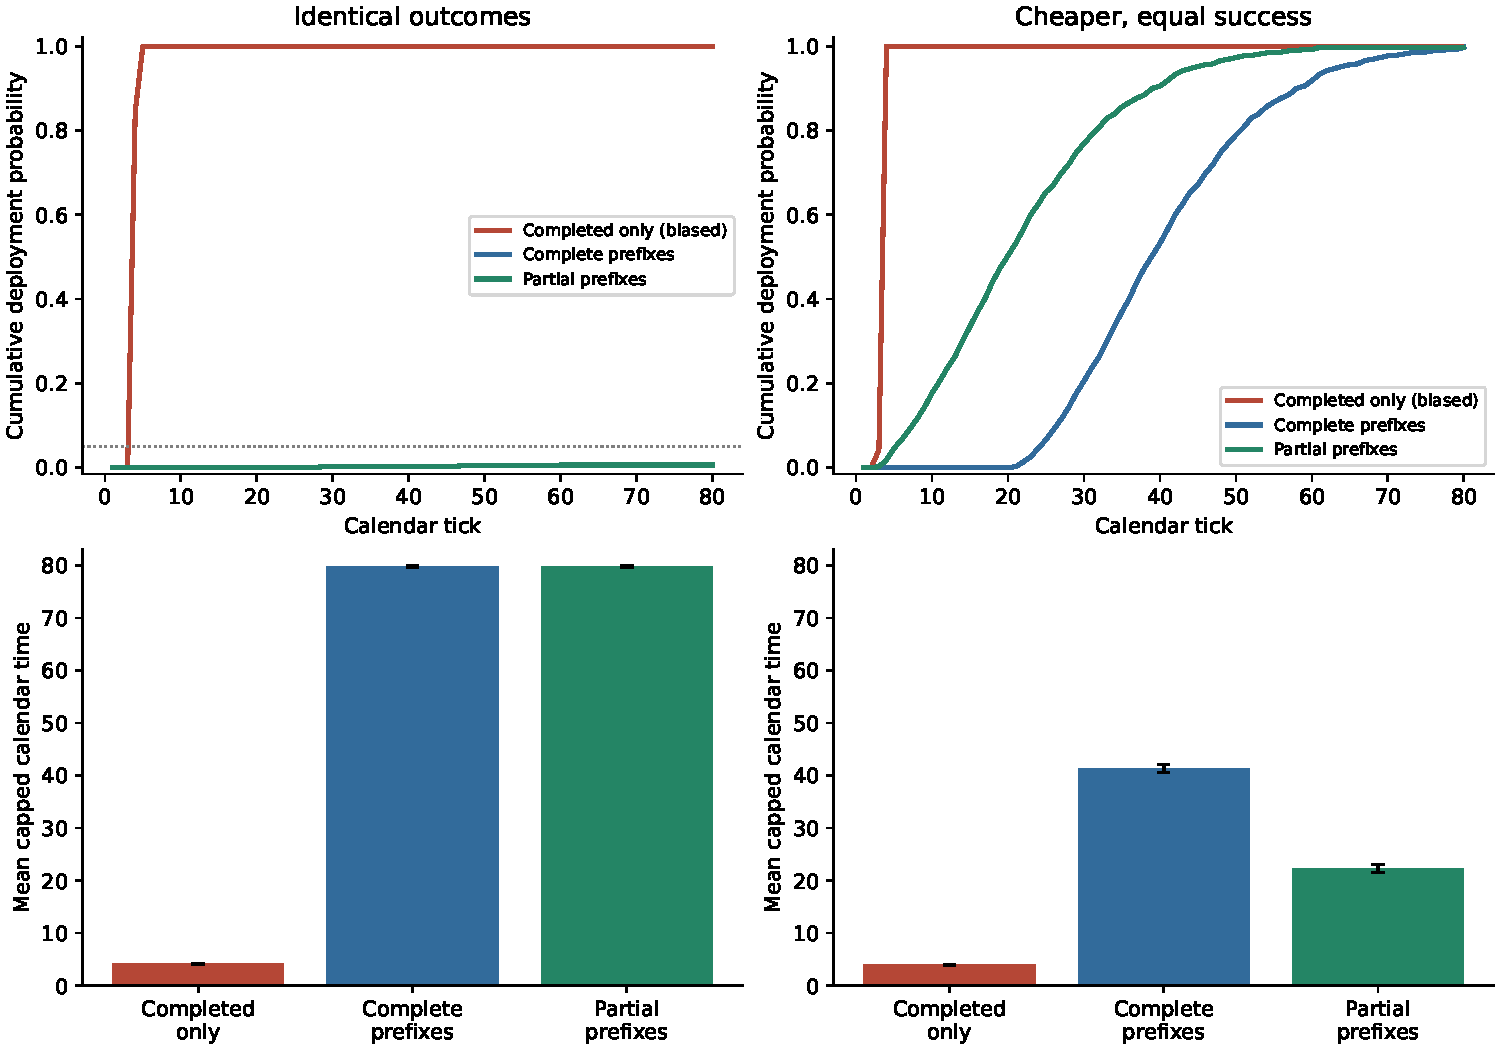
\includegraphics[width=\linewidth]{figures/async_operating.pdf}
\caption{Informative-delay score simulation. Partial-score prefix
inference retains the complete-data threshold guarantee while using
incomplete episodes. Completed-only selection targets a biased subset.
Calendar ticks and cost units are synthetic. Curves show the fraction
that has deployed, using the same latent draws for all methods.}
\label{fig:async}
\end{figure}
